\documentclass[12pt,a4paper]{article}
\usepackage{fontspec}
\setmainfont{Times New Roman}
\setsansfont{Arial}
\setmonofont{Consolas}
\usepackage[a4paper,top=25mm,bottom=25mm,left=30mm,right=25mm,headheight=15pt]{geometry}
\usepackage{setspace}\onehalfspacing
\usepackage{microtype,graphicx,booktabs,longtable,tabularx,array}
\graphicspath{{../figures/}}
\usepackage[table]{xcolor}
\usepackage{caption,enumitem,titlesec,fancyhdr}
\usepackage[hidelinks]{hyperref}
\usepackage{url,amsmath}
\definecolor{navy}{HTML}{17365D}
\definecolor{steel}{HTML}{4F81BD}
\definecolor{softgray}{HTML}{F2F2F2}
\definecolor{darkgray}{HTML}{4A4A4A}
\hypersetup{colorlinks=true,linkcolor=navy,citecolor=navy,urlcolor=steel,pdftitle={Therapeutic Target Landscape of Biologic Drugs in Autoimmune Disease},pdfauthor={Tharuniya Anpalakan}}
\titleformat{\section}{\Large\bfseries\color{navy}}{\thesection}{0.75em}{}
\titleformat{\subsection}{\large\bfseries\color{darkgray}}{\thesubsection}{0.75em}{}
\titleformat{\subsubsection}{\normalsize\bfseries\color{darkgray}}{\thesubsubsection}{0.75em}{}
\titlespacing*{\section}{0pt}{18pt}{8pt}
\pagestyle{fancy}\fancyhf{}
\fancyhead[L]{\small\textit{Therapeutic Target Landscape of Biologic Drugs}}
\fancyhead[R]{\small\textit{Tharuniya Anpalakan}}
\fancyfoot[C]{\thepage}\renewcommand{\headrulewidth}{0.4pt}
\captionsetup{font=normalsize,labelfont=bf,labelsep=period,justification=justified,singlelinecheck=false,skip=7pt}
\setlist{itemsep=2pt,topsep=5pt}\renewcommand{\arraystretch}{1.2}
\widowpenalty=10000
\clubpenalty=10000
\displaywidowpenalty=10000
\newcolumntype{Y}{>{\raggedright\arraybackslash}X}

\begin{document}
\begin{titlepage}
\thispagestyle{empty}\centering\vspace*{24mm}
{\color{navy}\rule{0.88\textwidth}{1.4pt}}\\[18mm]
{\fontsize{25}{31}\selectfont\bfseries\color{navy}Therapeutic Target Landscape of\\[3mm]Biologic Drugs in Autoimmune Disease\par}
\vspace{9mm}
{\large\color{darkgray}Molecular targets, immune pathways, clinical evidence,\\and reproducible network analysis\par}
\vspace{18mm}{\color{steel}\rule{0.42\textwidth}{0.8pt}}\\[16mm]
{\large\textbf{Author}\par}\vspace{4mm}
{\Large\textbf{Tharuniya Anpalakan}\par}\vspace{7mm}
{\large Department of Applied Sciences\par}
{\large Northumbria University\par}
{\large Newcastle upon Tyne, United Kingdom\par}\vspace{5mm}
{\large\href{mailto:w25070895@northumbria.ac.lk}{w25070895@northumbria.ac.lk}\par}
\vfill{\color{navy}\rule{0.88\textwidth}{1.4pt}}
\end{titlepage}

\pagenumbering{roman}
\section*{Abstract}\addcontentsline{toc}{section}{Abstract}
Biologic therapies have changed the treatment of immune-mediated disease by enabling intervention at defined cytokines, receptors, lymphocyte populations, immunoglobulin-recycling pathways, and complement components. The apparent precision of a molecular target, however, does not guarantee uniform clinical response. Disease heterogeneity, tissue-specific pathobiology, target redundancy, pharmacological architecture, and regulatory context all influence translation. This study developed a reproducible, evidence-linked landscape of 13 established or emerging biologics across rheumatoid arthritis, systemic lupus erythematosus and lupus nephritis, Sjögren disease, psoriatic arthritis, and generalized myasthenia gravis. Eleven direct human protein targets and 16 verified drug--target relationships were curated with indication-specific clinical and regulatory evidence. A heterogeneous NetworkX graph integrated drugs, molecular targets, diseases, and pathway systems through typed relationships that distinguish direct targeting, pathway participation, clinical investigation, and approval.

The resulting network comprised 39 nodes and 40 edges. Shared-target patterns were concentrated around TNF, CD20, and IL-17A/IL-17F, whereas FcRn, C5, BAFF receptor, and CD40 ligand represented more specialized mechanisms in this selected landscape. Descriptive pathway mapping identified TNF/NF-\(\kappa\)B signaling, B-cell depletion and survival, IL-6 signaling, IL-17 signaling, IgG homeostasis, terminal complement activation, and CD40 co-stimulation. Clinical evidence was examined separately from target evidence to prevent mechanistic plausibility from being interpreted as efficacy. The R4RA and STRAP trials illustrate both the promise and current limitations of synovial biomarker-guided treatment selection: molecular signals were observed, but a simple binary B-cell-rich/B-cell-poor classifier was not validated as a clinically reliable treatment-selection test. The project demonstrates how a compact, carefully audited dataset can provide a more defensible scientific resource than a larger collection with poorly resolved targets, indications, or approval states.

\noindent\textbf{Keywords:} autoimmune disease; biologic therapy; therapeutic targets; cytokines; B cells; FcRn; complement; precision medicine; network analysis; computational immunology.
\clearpage\tableofcontents\clearpage\listoffigures\clearpage\listoftables\clearpage\pagenumbering{arabic}

\section{Introduction}
Autoimmune diseases arise when mechanisms that maintain tolerance to self-antigens fail or become insufficient. The resulting pathology may involve autoreactive T cells, altered B-cell selection, autoantibody production, immune-complex deposition, complement activation, dysregulated cytokine networks, and persistent stromal or tissue-resident inflammatory programs. These mechanisms are not distributed uniformly across diseases or between patients with the same diagnosis. Rheumatoid arthritis (RA), for example, can contain lymphoid-rich, myeloid-rich, and comparatively pauci-immune synovial states; systemic lupus erythematosus (SLE) is characterized by considerable clinical and serological heterogeneity; and Sjögren disease combines glandular pathology with variable systemic involvement. A molecular target that is highly relevant in one biological context may therefore be less influential in another.

The clinical development of tumour necrosis factor (TNF) inhibitors established a durable model for targeted immunotherapy. Early studies showed that TNF could promote bone resorption, inhibit bone formation, and drive cartilage degradation \cite{bertolini1986,saklatvala1986}. Work in rheumatoid synovial cultures positioned TNF upstream of part of the inflammatory cytokine cascade \cite{brennan1989}. Anti-TNF treatment then reduced established disease in murine collagen-induced arthritis \cite{williams1992}. These experiments supplied mechanistic and preclinical justification, but human trials were required to determine efficacy, dosage, immunogenicity, and infection risk. The sequence remains instructive: target validation is an evidence chain rather than a single observation.

The modern therapeutic landscape extends beyond cytokine neutralization. B-cell-directed therapies deplete CD20-positive cells or interrupt BAFF/APRIL survival signaling; IL-17 inhibitors neutralize related effector cytokines; FcRn blockade accelerates IgG degradation; complement inhibitors act downstream of autoantibody binding; and CD40L antagonists interrupt co-stimulatory communication. Engineered antibodies, Fc fragments, receptor-Fc fusion proteins, and VHH nanobodies further demonstrate that modality and mechanism cannot be treated as interchangeable categories.

This report integrates these relationships in an auditable computational framework. The objective is not to rank treatments or provide patient-specific recommendations. Instead, it asks how direct molecular interactions, disease contexts, pathway membership, regulatory state, and clinical evidence can be represented without conflating fundamentally different types of evidence.

\section{Research Questions and Objectives}
The primary research question was:
\begin{quote}\textit{How can the molecular targets, immune pathways, and clinical evidence of established and emerging biologic therapies for autoimmune diseases be systematically mapped and compared using reproducible computational methods?}\end{quote}
The study addressed five measurable objectives:
\begin{enumerate}
\item curate a focused catalog of biologics with explicit modality, target, indication, jurisdiction, regulatory state, verification date, and evidence source;
\item validate direct human protein targets using standardized gene symbols and UniProt accessions;
\item construct a typed drug--target--disease--pathway network that preserves the difference between approval and investigation;
\item summarize pathway and clinical-evidence coverage without inappropriate enrichment tests or cross-trial efficacy rankings; and
\item evaluate molecularly guided biologic selection using R4RA and STRAP as focused case studies.
\end{enumerate}

\section{Immunological and Pharmacological Background}
\subsection{Immune tolerance and chronic tissue injury}
Central tolerance removes or edits many high-affinity autoreactive lymphocytes during development, whereas peripheral tolerance restrains cells that escape into the circulation. Anergy, deletion, inhibitory receptors, regulatory T cells, restricted co-stimulation, and anatomical sequestration all contribute. Autoimmune pathology can emerge when genetic susceptibility, infection, tissue damage, hormonal influences, environmental exposure, or stochastic immune events disturb these safeguards. B cells contribute through antibody production, antigen presentation, cytokine release, and organization of lymphoid structures. T cells provide help to B cells and macrophages, supply inflammatory cytokines, and in some conditions directly injure tissue.

Autoantibodies can be biomarkers, pathogenic mediators, or both. They may block or stimulate receptors, form immune complexes, recruit Fc-receptor-bearing cells, or activate complement. Complement fragments promote inflammation and opsonization, while the terminal cascade can damage susceptible membranes. Chronic inflammation also alters stromal cells and tissue architecture; accordingly, removal of a circulating cytokine or lymphocyte population may not immediately reverse an established local program.

\subsection{TNF, TNFR1, TNFR2, and inflammatory signaling}
TNF is produced as a membrane protein and can be released as a soluble ligand following proteolytic processing. Signaling through TNFR1 and TNFR2 is context dependent. TNFR1 is widely expressed and can activate canonical NF-\(\kappa\)B and MAPK pathways, promote survival, or initiate cell-death programs. TNFR2 is more restricted and is particularly relevant to immune-cell activation, tissue repair, and regulatory functions. Consequently, the clinical action of TNF blockade cannot be reduced to a single linear signaling arrow.

Infliximab and adalimumab are antibodies that neutralize TNF. Etanercept is a soluble TNF-receptor-Fc fusion that acts as a decoy receptor and has a distinct binding profile. The three agents therefore share a principal curated target while differing in molecular architecture and pharmacological behavior. Their shared target produces a prominent hub in the evidence graph, but that graph property should not be interpreted as superior efficacy.

\subsection{B-cell depletion and BAFF/APRIL biology}
CD20, encoded by \textit{MS4A1}, is present on many mature B-cell stages but is absent from most long-lived plasma cells. Rituximab is a type I anti-CD20 monoclonal antibody, whereas obinutuzumab is a glycoengineered type II antibody developed to enhance direct cell death and Fc-mediated effector activity. The phase II NOBILITY program and subsequent phase III REGENCY evidence supported obinutuzumab in active lupus nephritis \cite{furie2022nobility,furie2025regency}. Its mechanism remains broader than selective deletion of autoreactive clones because protective CD20-positive B cells are also depleted.

BAFF promotes B-cell survival through receptors including BAFF-R, while APRIL shares TACI and BCMA as receptors in relevant B-cell and plasma-cell contexts. Ianalumab combines BAFF-R blockade with antibody-dependent B-cell depletion. A phase IIb Sjögren study reported dose-related biological and clinical signals that justified phase III development \cite{bowman2022}. Telitacicept is a TACI-Fc fusion protein that sequesters both BAFF and APRIL. A China-based phase III SLE trial demonstrated improvement in the prespecified composite response, but jurisdiction and population remain important when interpreting regulatory and generalizability claims \cite{vollenhoven2025}.

\subsection{IL-17A and IL-17F blockade}
IL-17A and IL-17F form homo- and heterodimers that signal through IL-17 receptor complexes. Their downstream programs promote chemokines, antimicrobial mediators, granulocyte recruitment, and tissue inflammation. Bimekizumab neutralizes both cytokines. Phase III psoriatic arthritis trials demonstrated improvement relative to placebo in biologic-naive and TNF-inhibitor-experienced populations \cite{mcinnes2023,merola2023}. Oral candidiasis and other fungal infections are biologically coherent safety observations because IL-17 contributes to mucosal antifungal defense.

Sonelokimab is a multivalent VHH construct containing IL-17A-binding, IL-17F-binding, and albumin-binding domains. It illustrates how modular antibody fragments can combine dual cytokine recognition with exposure-extending design. Phase II evidence in psoriatic arthritis supports continued development, but does not establish superiority over approved monoclonal antibodies \cite{mcinnes2025}.

\subsection{FcRn and IgG homeostasis}
FcRn binds IgG within acidic endosomes, protects it from lysosomal degradation, and releases it after recycling to the neutral extracellular environment. Efgartigimod is an engineered Fc fragment with enhanced FcRn affinity under conditions that competitively interrupt recycling. IgG is consequently directed toward degradation, reducing both pathogenic and protective circulating IgG. ADAPT demonstrated clinical benefit in generalized myasthenia gravis, particularly within its prespecified AChR-antibody-positive population \cite{howard2021}. FcRn inhibition does not eliminate antibody-producing cells, and IgG can recover after treatment cycles. Reviews emphasize the need to resolve optimal scheduling, long-term infection risk, and indication-specific selection \cite{patel2024fcrn,mohamed2024fcrn}.

\subsection{Complement C5 inhibition}
The classical, lectin, and alternative complement pathways converge on C5 cleavage. C5a is a potent inflammatory mediator, while C5b initiates membrane-attack-complex assembly. Ravulizumab is a long-acting C5 antibody engineered from eculizumab. In AChR-antibody-positive generalized myasthenia gravis, it acts downstream of pathogenic antibody binding. CHAMPION-MG reported improvement in disease activity \cite{vu2022}. Because C5 blockade compromises terminal complement defense, meningococcal infection risk and prevention are central to clinical use.

\subsection{CD40--CD40L co-stimulation}
CD40L is expressed predominantly by activated T cells and binds CD40 on B cells and antigen-presenting cells. The interaction supports B-cell activation, germinal-centre organization, class switching, and memory development. Dazodalibep is a non-antibody fusion protein that antagonizes CD40L. A randomized phase II study in Sjögren disease reported signals in two prospectively defined populations \cite{stclair2024}. These findings justify phase III evaluation, but do not establish routine effectiveness, durable remission, or approval.

\section{Materials and Methods}
\subsection{Source review and evidence selection}
The starting document was reviewed for candidate agents, molecular targets, diseases, clinical studies, and figures. It was not treated as a scientific authority. Administrative content, branding, assessment declarations, and images with unclear reuse rights were excluded from analytical outputs. The unchanged source is maintained separately from public version control.

Evidence was accepted when a direct target, disease context, and traceable source could be identified. Regulatory status was recorded per indication, jurisdiction, and verification date. An approval in one disease or jurisdiction was not propagated to another. Primary clinical publications and regulatory product information were preferred over narrative summaries. UniProt and HGNC identifiers standardized protein and gene nomenclature.

\subsection{Data model}
Four linked tables supported the analysis. The biologic catalog used one row per drug--indication context. The target table stored gene symbols, protein names, UniProt accessions, HGNC identifiers, and target class. The drug--target evidence table used one row per verified direct relationship and preserved its interaction mechanism. The clinical-evidence table stored design, phase, sample size, comparator, endpoint, main finding, and limitation.

\begin{table}[htbp]\centering
\caption{Core evidence tables and their analytical purpose.}\label{tab:data-model}
\begin{tabularx}{\textwidth}{>{\bfseries}p{0.27\textwidth}YY}\toprule
Table & Unit of observation & Principal safeguard \\\midrule
Biologic drug catalog & Drug--indication context & Status interpreted with jurisdiction and date \\
Therapeutic targets & Human protein target & Standardized gene and protein identifiers \\
Drug--target evidence & One direct interaction & Direct binding separated from downstream pathways \\
Clinical evidence & One selected study & Results not pooled across incompatible endpoints \\\bottomrule
\end{tabularx}\end{table}

\subsection{Validation and reproducibility}
Python validation tested required columns, duplicate rows, controlled verification states, and UniProt accession formatting. The analysis used relative paths and pinned package versions. Reusable functions were separated from notebooks. Synthetic fixtures were reserved for tests and were never mixed with research data. Ten automated tests evaluated table validation, target formatting, direct edge creation, regulatory relationship handling, disease mapping, clinical missingness, pathway membership, network metrics, and generation of all registered figures.

\subsection{Network construction}
A heterogeneous undirected graph was built with drug, target, disease, and pathway nodes. Four relationship classes were retained: direct targeting, approval for an indication, investigation for an indication, and participation in a pathway. The network is undirected for visualization; edge attributes retain semantic direction. Degree and components describe this evidence graph, not causal influence, biological indispensability, or comparative benefit.

\subsection{Pathway and clinical-evidence analysis}
Targets were mapped descriptively to eight immune systems: TNF/NF-\(\kappa\)B, B-cell depletion, IL-6 signaling, B-cell survival, IL-17 signaling, IgG homeostasis, terminal complement, and CD40 co-stimulation. Enrichment testing was not performed because the target set was small, manually selected, and non-random. Clinical studies were summarized by phase and disease. No meta-analysis or cross-disease ranking was attempted because populations, endpoints, comparators, background therapies, and follow-up differed materially.

\section{Results}
\subsection{Composition of the curated landscape}
The final dataset contained 13 unique biologics, 11 direct human protein targets, 16 direct drug--target relationships, and 10 selected clinical studies. Ten agents had an approval in the specific indication and jurisdiction represented. Ianalumab, sonelokimab, and dazodalibep remained investigational or designation-stage in the represented contexts. Telitacicept's approval was recorded specifically for SLE in China; it was not described as globally approved.

\begin{longtable}{p{0.18\textwidth}p{0.22\textwidth}p{0.20\textwidth}p{0.29\textwidth}}
\caption{Curated biologics, direct targets, and principal mechanisms.}\label{tab:agents}\\\toprule
\textbf{Agent} & \textbf{Modality} & \textbf{Direct target(s)} & \textbf{Curated mechanism} \\\midrule\endfirsthead
\toprule\textbf{Agent} & \textbf{Modality} & \textbf{Direct target(s)} & \textbf{Curated mechanism} \\\midrule\endhead
Infliximab & Chimeric mAb & TNF & Ligand neutralization \\
Adalimumab & Human mAb & TNF & Ligand neutralization \\
Etanercept & Receptor--Fc fusion & TNF & Soluble decoy-receptor binding \\
Rituximab & Chimeric mAb & CD20 & B-cell depletion \\
Tocilizumab & Humanized mAb & IL-6 receptor & Receptor blockade \\
Obinutuzumab & Glycoengineered type II mAb & CD20 & Enhanced B-cell cytolysis \\
Ianalumab & Human mAb & BAFF receptor & Receptor blockade and B-cell depletion \\
Telitacicept & TACI--Fc fusion & BAFF; APRIL & Dual ligand sequestration \\
Bimekizumab & Humanized mAb & IL-17A; IL-17F & Dual cytokine neutralization \\
Sonelokimab & Multivalent VHH & IL-17A; IL-17F & Nanobody cytokine neutralization \\
Efgartigimod & Engineered Fc fragment & FcRn & Competitive blockade of IgG recycling \\
Ravulizumab & Humanized mAb & C5 & Terminal complement inhibition \\
Dazodalibep & Domain fusion protein & CD40L & Co-stimulatory ligand antagonism \\\bottomrule
\end{longtable}

\subsection{Shared targets and network structure}
TNF was directly linked to three agents. CD20 was shared by rituximab and obinutuzumab. IL-17A and IL-17F were shared by bimekizumab and sonelokimab. Telitacicept and both IL-17-directed agents formed multi-target patterns. Other targets had one directly linked agent in the selected landscape. The integrated graph comprised 39 nodes and 40 edges. Drug--disease edges were labeled separately as approval or investigation relationships.

\begin{center}\begin{minipage}{0.98\textwidth}\centering
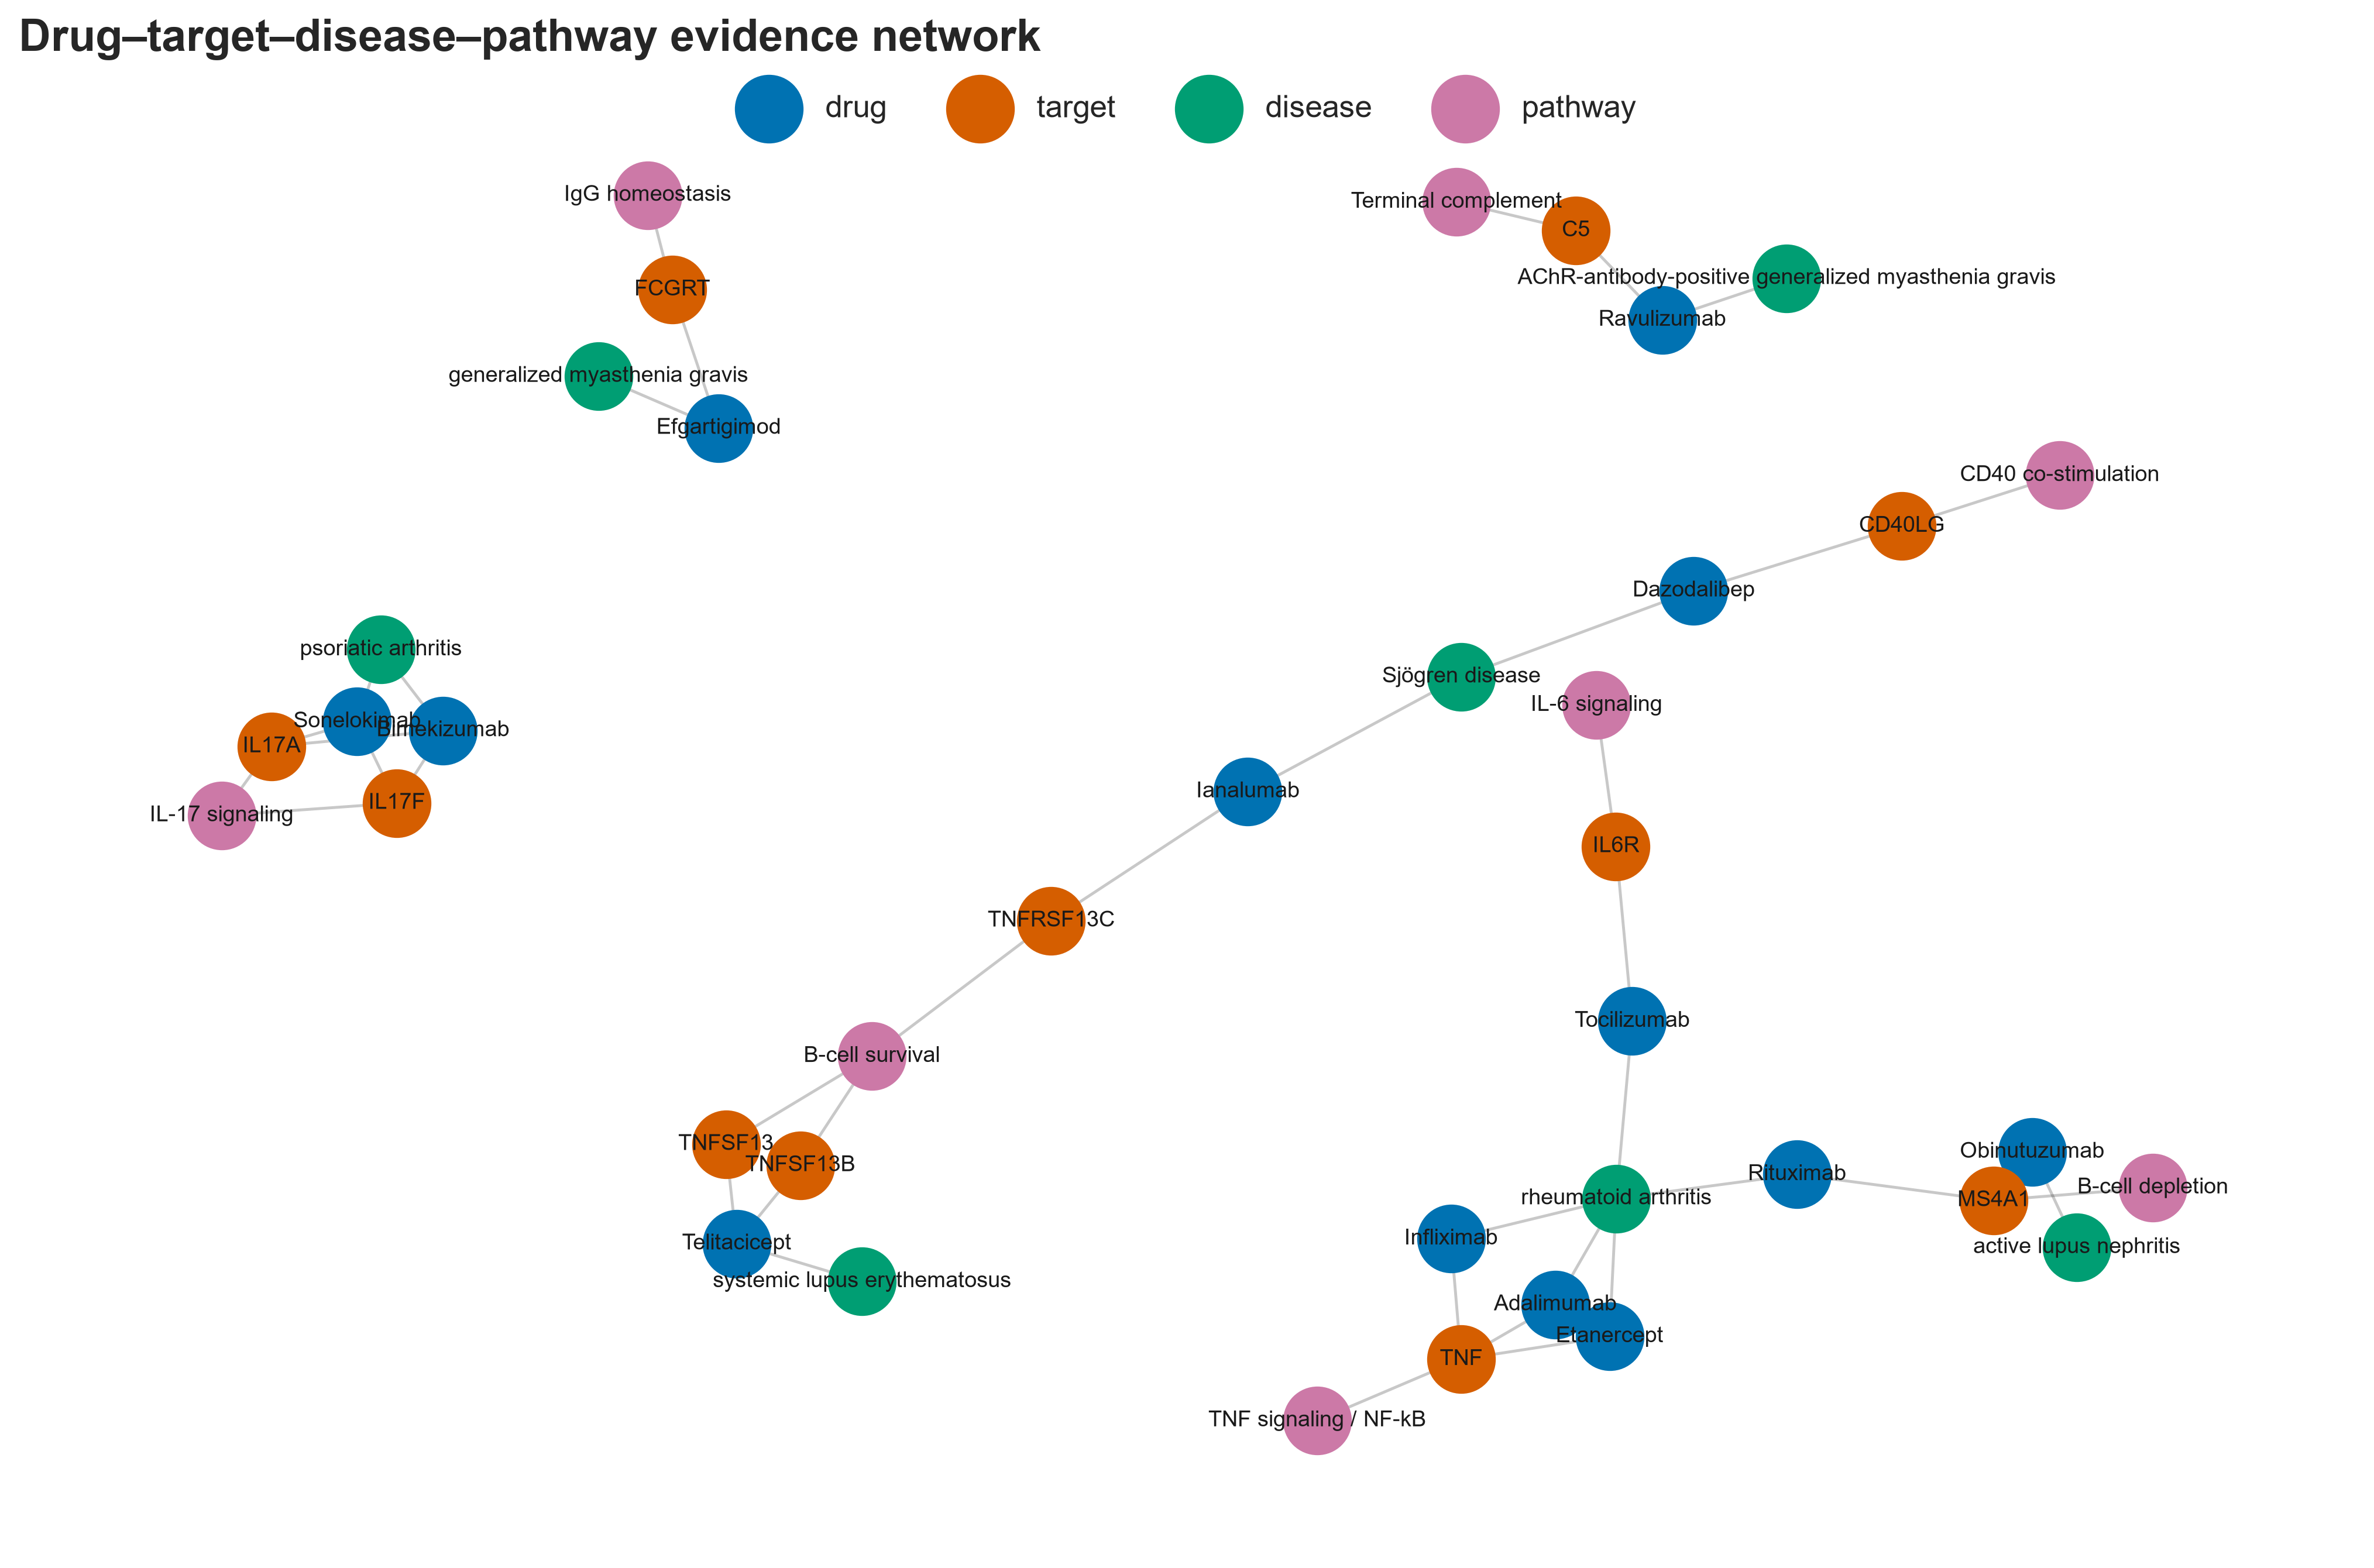
\includegraphics[width=0.96\textwidth,height=0.42\textheight,keepaspectratio]{figure_05_heterogeneous_network.png}
\captionof{figure}{Drug--target--disease--pathway evidence network. Blue nodes denote drugs, orange nodes direct targets, green nodes diseases, and purple nodes pathway systems. Spatial proximity is produced by the layout algorithm and is not a measure of clinical similarity.}\label{fig:network}
\end{minipage}\end{center}

\subsection{Drug--target evidence matrix}
The evidence matrix makes shared targets and agent-specific mechanisms explicit. A marked cell denotes a documented direct relationship. An unmarked cell means that no direct interaction was documented within this scope; it is not experimental evidence that an interaction is impossible.
\begin{center}\begin{minipage}{0.98\textwidth}\centering
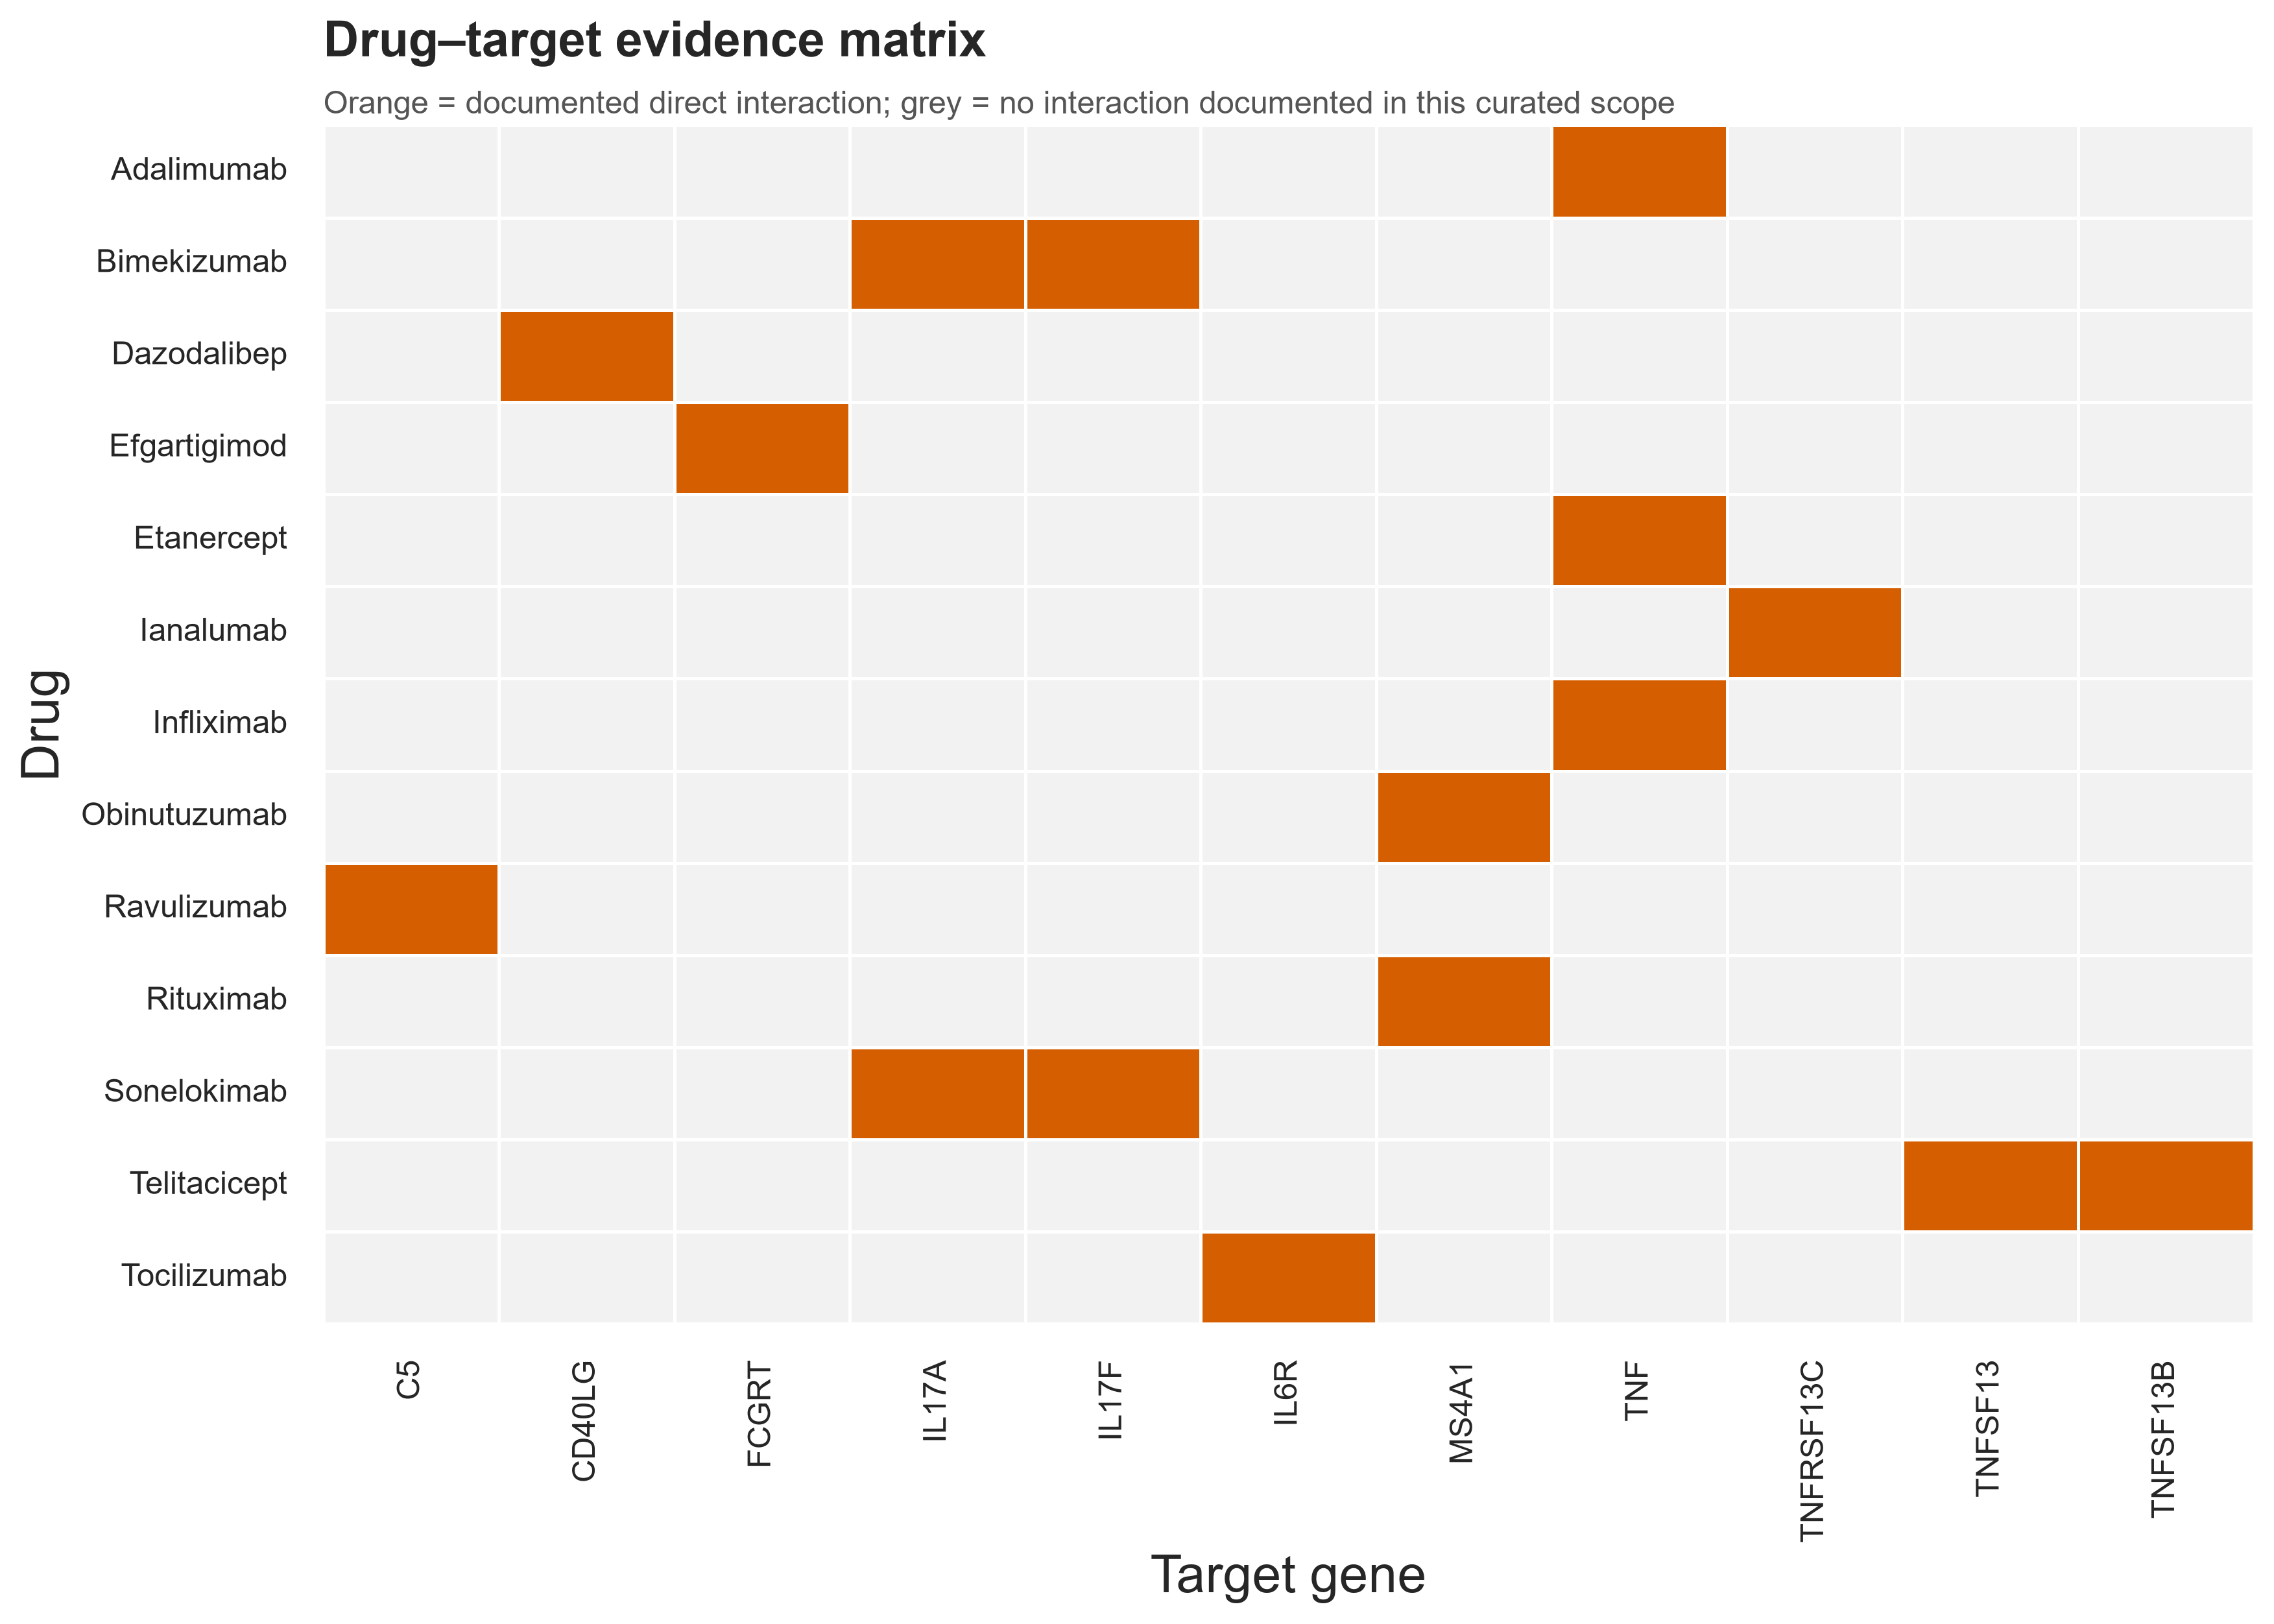
\includegraphics[width=0.96\textwidth,height=0.36\textheight,keepaspectratio]{figure_04_drug_target_heatmap.png}
\captionof{figure}{Direct drug--target association matrix. Orange cells represent verified direct interactions. Grey cells represent absence of documented direct evidence in the current dataset.}\label{fig:matrix}
\end{minipage}\end{center}

\subsection{Pathway coverage}
The pathway matrix showed broad mechanistic diversity despite the compact dataset. TNF, IL-6, and IL-17 represented cytokine intervention; CD20, BAFF-R, BAFF, and APRIL represented B-cell depletion or survival; FcRn represented antibody homeostasis; C5 represented downstream effector blockade; and CD40L represented interruption of co-stimulation. Target membership alone did not encode mechanism. A receptor-blocking biologic binds a cell-surface receptor and prevents signalling, whereas a soluble receptor-based decoy, such as etanercept, sequesters its ligand before that ligand reaches a signalling receptor. Other agents in the dataset neutralized ligands, depleted target-bearing cells, or altered antibody recycling.
\begin{center}\begin{minipage}{0.98\textwidth}\centering
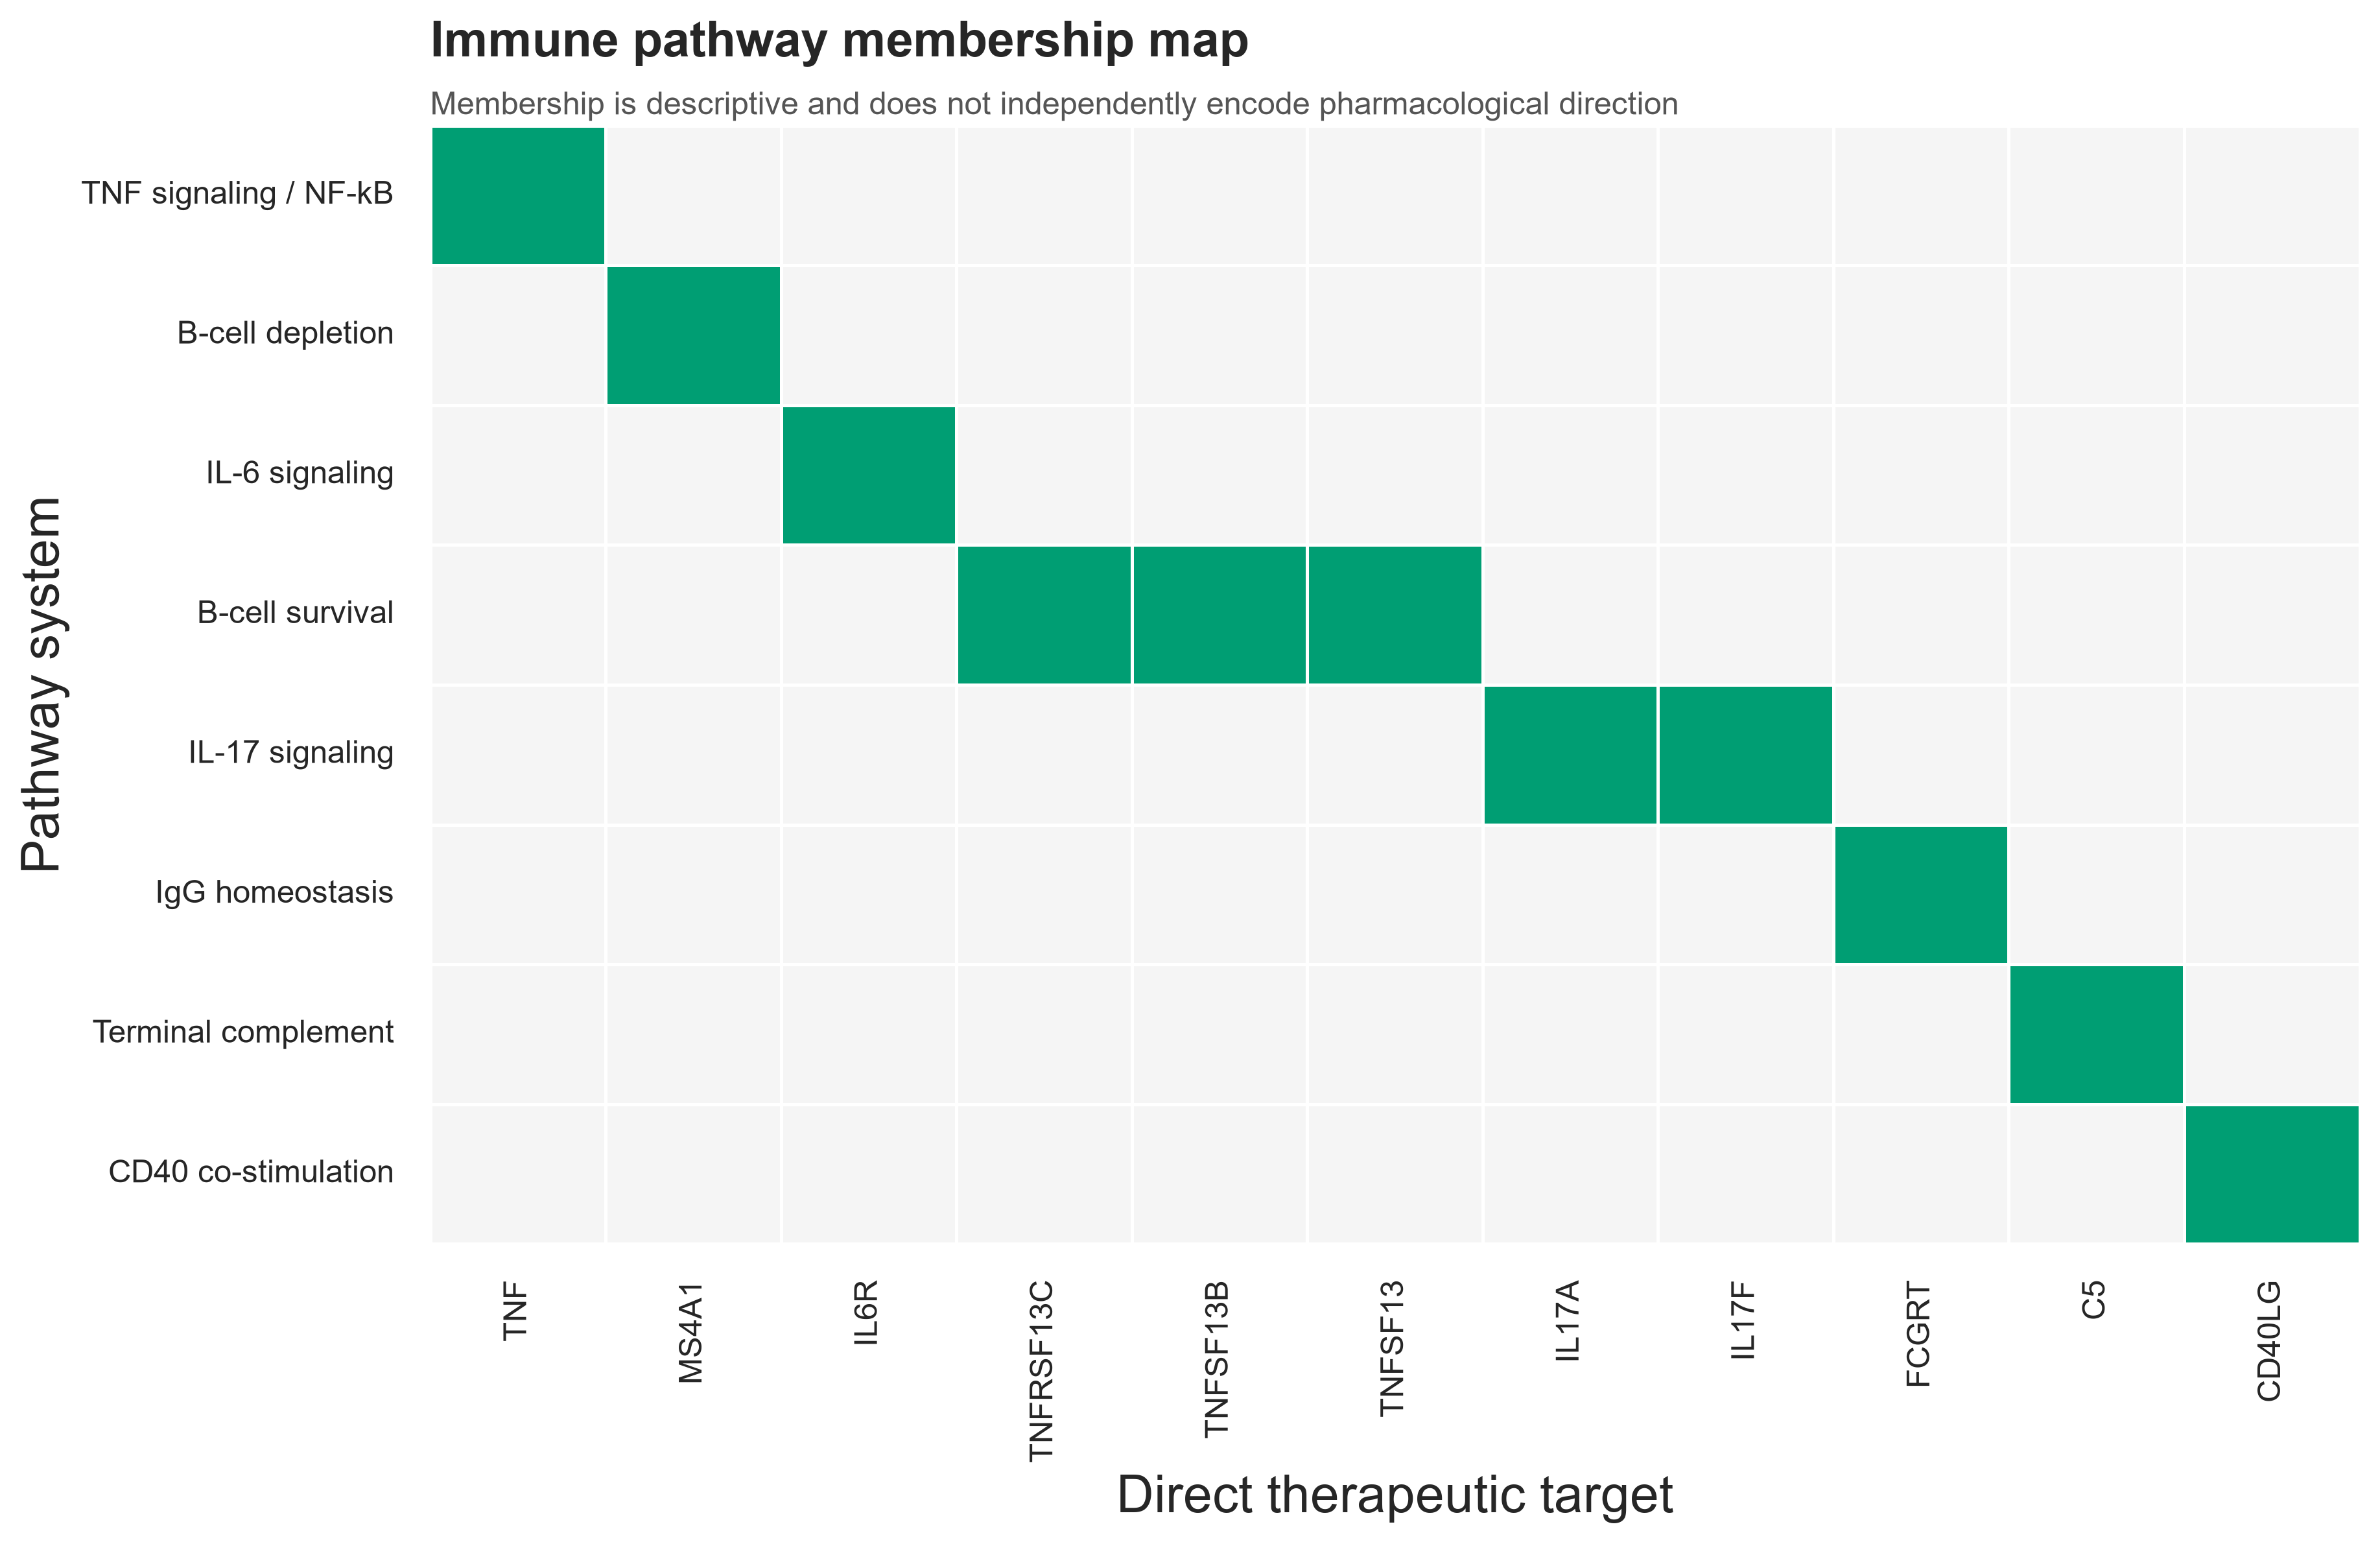
\includegraphics[width=0.94\textwidth,height=0.34\textheight,keepaspectratio]{figure_06_pathway_map.png}
\captionof{figure}{Descriptive target--pathway membership matrix. Membership does not independently infer the direction or magnitude of pharmacological effect.}\label{fig:pathways}
\end{minipage}\end{center}

\subsection{Clinical-evidence coverage}
The selected set included phase II, III, and IV studies. Phase III evidence predominated because several agents were established therapies or had recently completed pivotal development. Study counts should not be interpreted as evidence strength without considering design, population, endpoint, and replication.
\begin{center}\begin{minipage}{0.98\textwidth}\centering
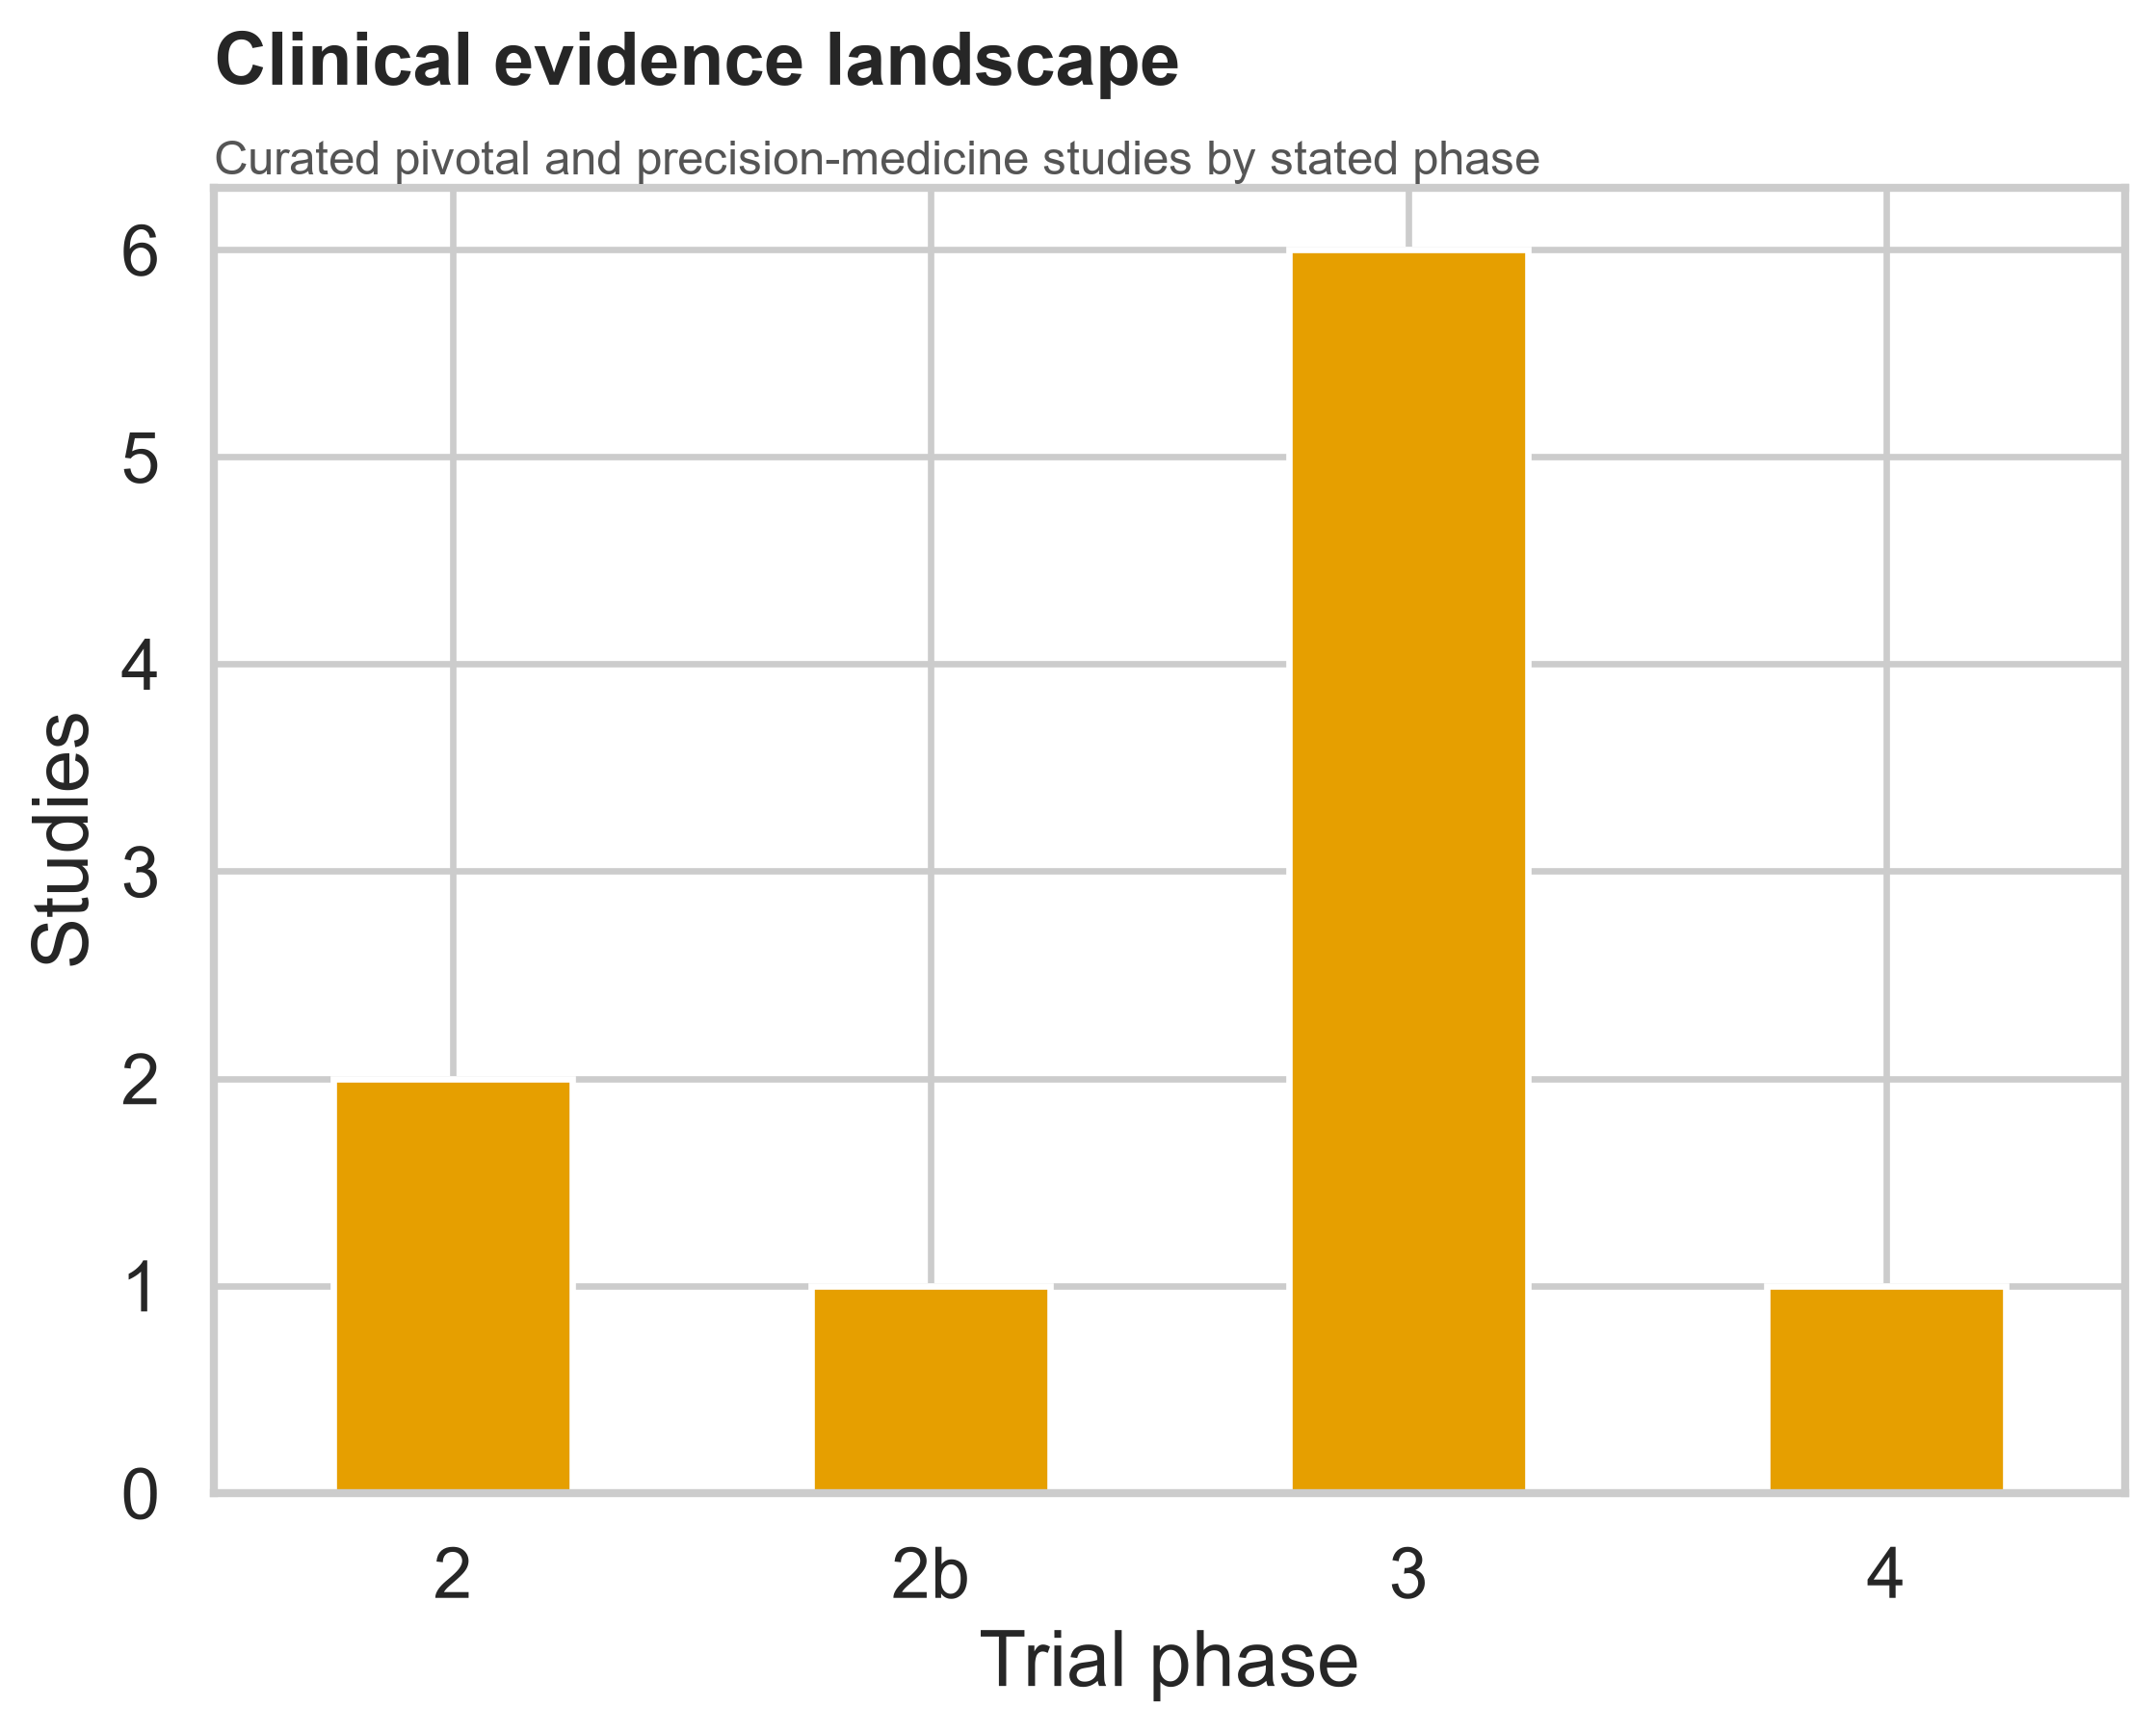
\includegraphics[width=0.72\textwidth,height=0.36\textheight,keepaspectratio]{figure_08_clinical_evidence.png}
\captionof{figure}{Distribution of the ten selected clinical studies by phase. The figure describes evidence coverage and does not compare efficacy.}\label{fig:clinical}
\end{minipage}\end{center}

\section{Precision Immunotherapy: R4RA and STRAP}
\subsection{R4RA}
R4RA enrolled 164 patients with RA who had an inadequate response to TNF inhibition and randomized them to rituximab or tocilizumab following synovial biopsy \cite{humby2021}. The histology-defined primary comparison did not show a significant treatment difference. When B-cell status was defined using a molecular signature, a differential signal favoring tocilizumab in the B-cell-low group was observed. This discrepancy is important: biomarker performance depends on assay platform, threshold, reproducibility, and prespecified analysis.

\subsection{STRAP}
STRAP and STRAP-EU evaluated rituximab, tocilizumab, and etanercept in 226 biologic-naive patients after synovial biopsy \cite{rivellese2024}. In the B-cell-poor primary population, week-16 ACR20 response was similar between grouped etanercept/tocilizumab and rituximab. The prespecified binary classifier therefore did not predict differential response. Later transcriptomic analyses identified multigene response signatures and reported cross-cohort validation \cite{rivellese2025}. These results advance biomarker development, but retrospective accuracy is not equivalent to prospective clinical utility.

\subsection{Implications for biomarker development}
A clinically useful predictive biomarker must add information beyond routine variables, operate reproducibly across laboratories, and improve outcomes when used to assign treatment. It also requires prospective validation of the complete decision rule. Tissue sampling introduces challenges: one joint may not represent all joints, cellular composition varies within tissue, and RNA signatures may change with treatment or disease duration. R4RA and STRAP support continued tissue-based investigation while arguing against premature adoption of a simple binary classifier.
\begin{center}\begin{minipage}{0.98\textwidth}\centering
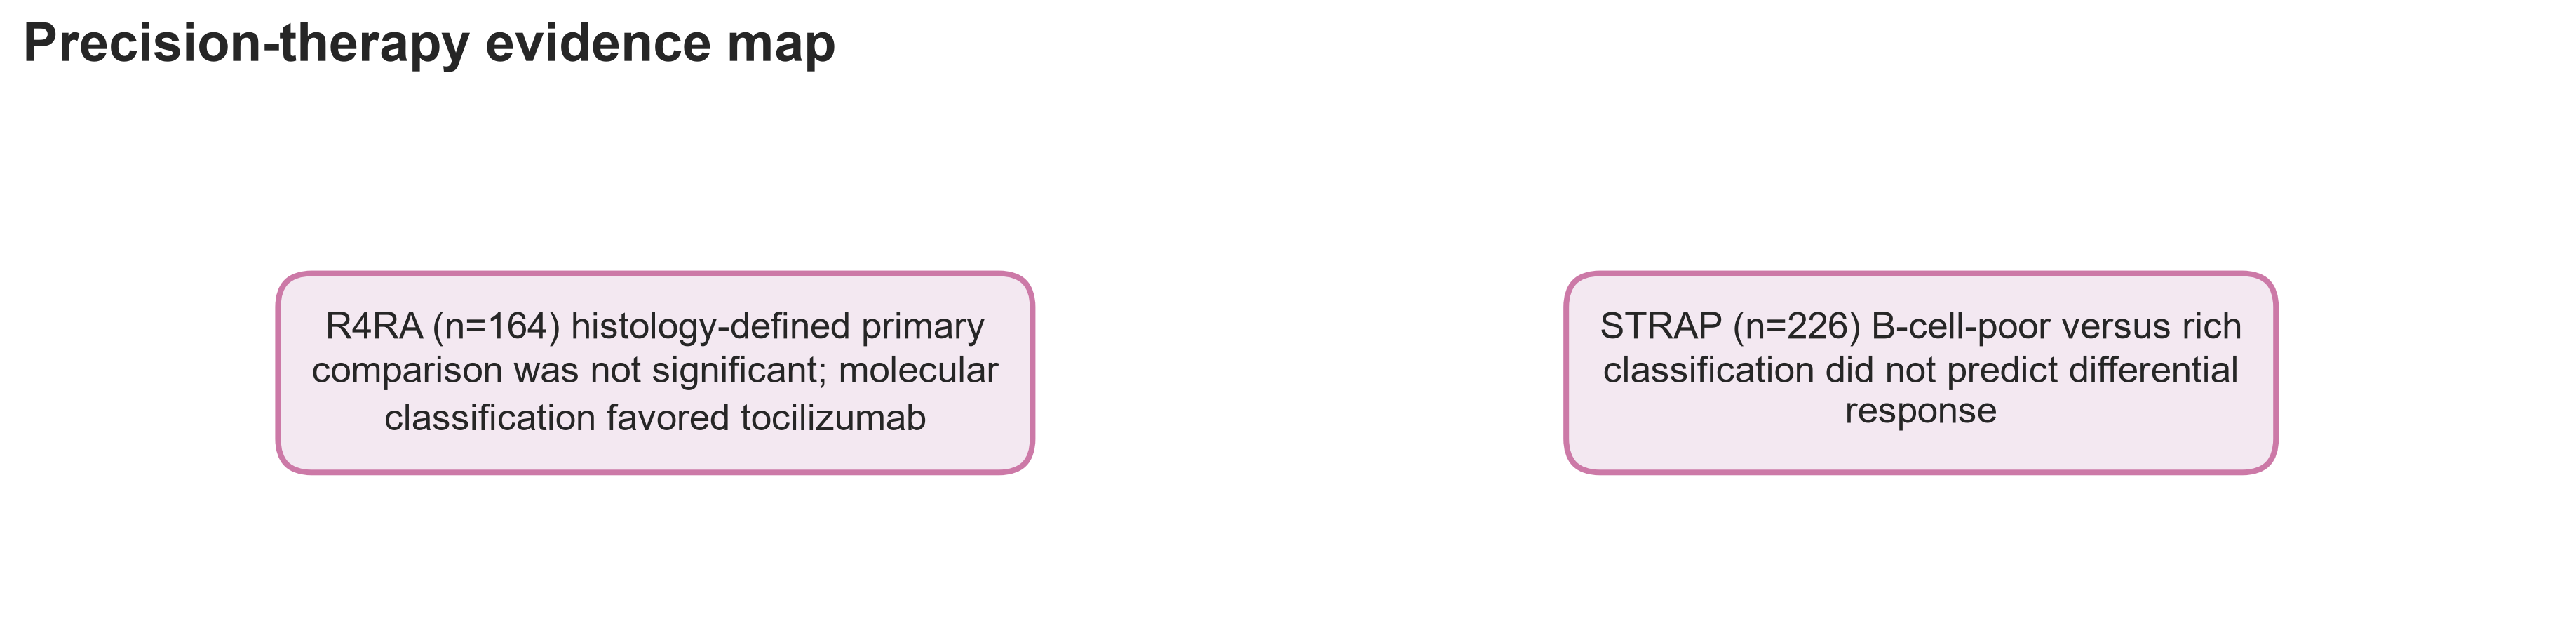
\includegraphics[width=0.93\textwidth,height=0.31\textheight,keepaspectratio]{figure_09_precision_evidence.png}
\captionof{figure}{Precision-treatment evidence map for R4RA and STRAP. The studies establish the feasibility and biological value of synovial profiling but do not validate a routine companion diagnostic.}\label{fig:precision}
\end{minipage}\end{center}

\section{Biologic Modality and Molecular Engineering}
Conventional monoclonal antibodies provide bivalent recognition and an Fc domain capable of influencing half-life and effector function. Glycoengineering can modify Fc-receptor interactions, as illustrated by obinutuzumab. Receptor-Fc fusion proteins present an extracellular receptor domain as a soluble trap; etanercept and telitacicept use this architecture for different ligand systems. Engineered Fc fragments such as efgartigimod exploit FcRn biology without antigen-binding variable domains. VHH nanobodies are smaller single-domain binders that can be linked modularly, as in sonelokimab. Dazodalibep uses a CD40-binding-domain fusion and is not a conventional antibody.

These structural categories affect valency, distribution, recycling, effector recruitment, manufacturing, and potential immunogenicity. They do not, in isolation, demonstrate superior clinical performance. Reliable comparison requires direct studies with appropriate endpoints and populations.
\begin{center}\begin{minipage}{0.98\textwidth}\centering
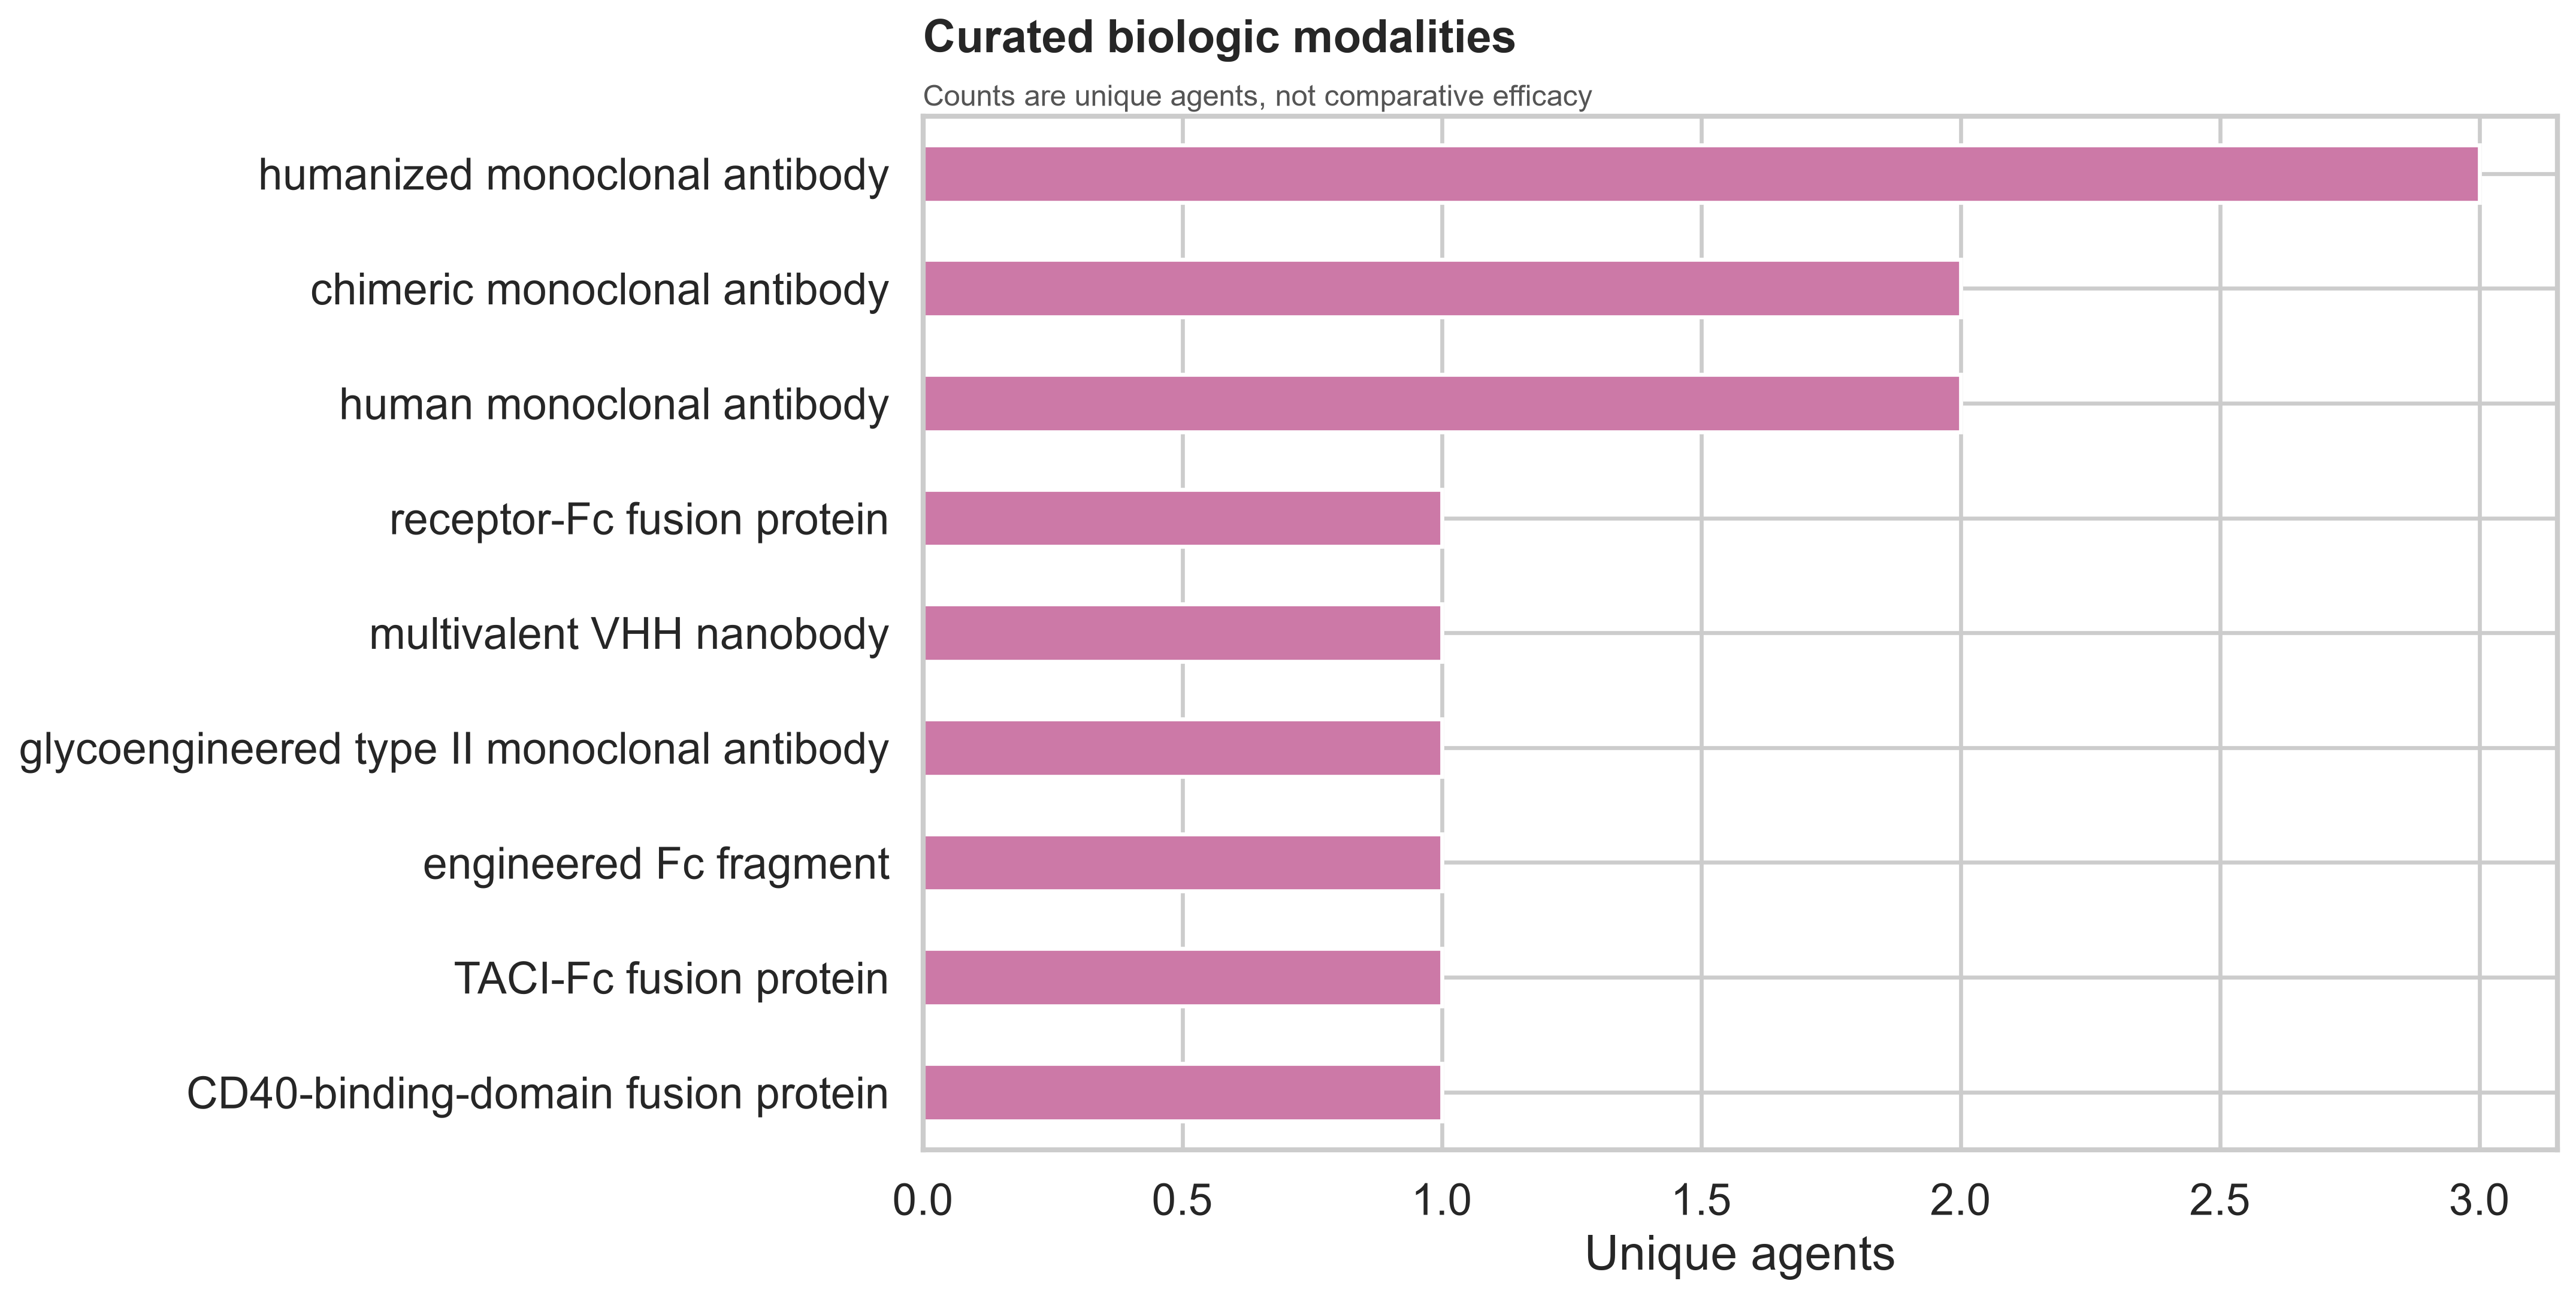
\includegraphics[width=0.84\textwidth,height=0.34\textheight,keepaspectratio]{figure_07_modality_comparison.png}
\captionof{figure}{Distribution of molecular modalities. Counts describe structural diversity and should not be interpreted as comparative effectiveness.}\label{fig:modality}
\end{minipage}\end{center}

\section{Emerging Therapeutic Platforms}
\subsection{Antigen-specific tolerance and delivery systems}
Antigen-specific therapy seeks to suppress responses to disease-relevant antigens while preserving broader host defense. Nanoparticles can co-deliver antigen and tolerogenic signals. In experimental autoimmune encephalomyelitis, dual-peptide PLGA systems reduced inflammatory T-cell responses and demyelination \cite{wang2022nano}. Translation is constrained by uncertainty about dominant human autoantigens, epitope spreading, formulation reproducibility, and differences between induced animal models and established human disease.

Biomimetic vesicles, electrospun fibers, hydrogels, and microneedle systems may localize treatment or alter release kinetics. Preclinical arthritis studies have reported antioxidant nanohybrids and microneedle approaches \cite{koo2023,xia2024}. Such platforms must preserve biologic conformation, potency, sterility, and batch consistency. Local delivery also faces anatomical differences between superficial animal joints and deeper human joints.

\subsection{CAR-T-cell approaches}
CAR-T therapy is a cellular intervention and should not be classified as an antibody drug, even though its receptor contains antibody-derived recognition domains. CD19-directed CAR-T cells can produce deep B-cell depletion and have generated remissions in small, severe autoimmune-disease series \cite{muller2024}. Dual CD19/BCMA approaches additionally seek to target plasma-cell compartments; early phase I evidence in SLE and lupus nephritis is encouraging but uncontrolled and small \cite{wang2024cart}. Lymphodepletion, cytokine-release syndrome, infection, manufacturing complexity, cost, and long-term surveillance remain substantial considerations.

\section{Discussion}
The central finding is that a useful therapeutic landscape depends on typed evidence. A drug can bind a protein directly, influence a pathway indirectly, be investigated in a disease, or be approved for a specific indication. These relationships are not interchangeable. When collapsed, an evidence map can overstate clinical maturity or imply mechanisms not demonstrated by binding evidence.

The network identifies areas of convergence. TNF, CD20, and IL-17A/F connect multiple agents, reflecting both target validation and alternative architectures. Conversely, FcRn, C5, BAFF-R, and CD40L occupy more specialized positions. Low degree does not mean low biological importance; it may reflect novelty, narrow selection, or fewer agents in the dataset.

The separation of mechanism and efficacy is equally important. A well-validated target can fail to predict response because disease activity is sustained by redundant pathways, tissue states, irreversible damage, inadequate exposure, or differences in clinical endpoints. R4RA and STRAP show why molecular stratification must be evaluated as a complete diagnostic strategy. Later transcriptomic work is meaningful, yet prospective assignment studies remain necessary.

Regulatory context adds another layer. Obinutuzumab's lupus-nephritis approval, telitacicept's China-specific SLE approval, and designation-stage ianalumab cannot be summarized accurately with one global status field. The catalog therefore preserves indication, jurisdiction, and verification date. This design is more verbose but scientifically safer.

\section{Translational Implications}
Evidence-linked maps can support target prioritization, trial-design review, identification of shared pathways, and recognition of gaps. They can guide questions about sequencing or combination, but cannot select therapy for an individual. Clinical choice depends on diagnosis, prior treatment, comorbidity, infection risk, vaccination, pregnancy considerations, route, monitoring, access, and patient preference.

Future development should connect tissue and circulating biomarkers to longitudinal outcomes, integrate multi-omic measurements with interpretable models, and test assignment rules prospectively. Mechanistic studies should distinguish pharmacodynamic target engagement from clinical response. For emerging modalities, comparative evidence should address whether engineering produces a clinically meaningful advantage rather than only a structural change.

\section{Limitations}
The landscape is purposive rather than exhaustive. It prioritizes 13 agents from the source context and does not represent every licensed autoimmune biologic. One principal indication per agent simplifies extensive multi-disease labels. Regulatory status can change and differs across countries. Broad pathway categories are interpretive summaries rather than complete event hierarchies. The graph is undirected and does not model dose, tissue concentration, time, target expression, or causality. Manual curation can introduce error despite validation. Trial heterogeneity prevented meta-analysis and comparative ranking. The dataset is an auditable landscape, not a clinical decision system.

\section{Conclusion}
This study developed a reproducible landscape connecting 13 biologic agents, 11 direct protein targets, 16 verified interactions, five principal disease contexts, eight pathway systems, and ten selected clinical studies. The analysis shows how apparently similar therapies differ in architecture and mechanism, and how shared targets coexist with disease-specific evidence and regulation. It also demonstrates that precision immunotherapy remains an empirical challenge: molecular profiling can reveal meaningful heterogeneity, but predictive utility requires more than association.

The principal contribution is a transparent evidence structure in which direct target binding, pathway participation, clinical investigation, and approval remain distinct. That structure provides a defensible foundation for future expansion, regulatory updates, and prospective biomarker research.

\section*{Reproducibility Statement}\addcontentsline{toc}{section}{Reproducibility Statement}
The project was executed with Python 3.14.2 using pinned versions of pandas, NumPy, NetworkX, Matplotlib, seaborn, nbformat, nbclient, and pytest. Seven notebooks were executed with saved outputs and ten automated tests passed. The analysis is regenerated by running the pipeline module and then the notebook-execution script, as documented in the repository README. This report is compiled from the present \LaTeX{} source using XeLaTeX and the installed Times New Roman font.

\begin{thebibliography}{99}\addcontentsline{toc}{section}{References}
\bibitem{bertolini1986} Bertolini DR, Nedwin GE, Bringman TS, Smith DD, Mundy GR. Stimulation of bone resorption and inhibition of bone formation in vitro by human tumour necrosis factors. \textit{Nature}. 1986;319:516--518. doi:10.1038/319516a0.
\bibitem{saklatvala1986} Saklatvala J. Tumour necrosis factor-\(\alpha\) stimulates resorption and inhibits synthesis of proteoglycan in cartilage. \textit{Nature}. 1986;322:547--549. doi:10.1038/322547a0.
\bibitem{brennan1989} Brennan FM, Chantry D, Jackson A, Maini R, Feldmann M. Inhibitory effect of TNF-\(\alpha\) antibodies on synovial cell interleukin-1 production in rheumatoid arthritis. \textit{Lancet}. 1989;334:244--247. doi:10.1016/S0140-6736(89)90430-3.
\bibitem{williams1992} Williams RO, Feldmann M, Maini RN. Anti-tumor necrosis factor ameliorates joint disease in murine collagen-induced arthritis. \textit{PNAS}. 1992;89:9784--9788. doi:10.1073/pnas.89.20.9784.
\bibitem{jung2022} Jung SM, Kim WU. Targeted immunotherapy for autoimmune disease. \textit{Immune Network}. 2022;22:e9. doi:10.4110/in.2022.22.e9.
\bibitem{furie2022nobility} Furie RA, Aroca G, Cascino MD, et al. B-cell depletion with obinutuzumab for proliferative lupus nephritis. \textit{Ann Rheum Dis}. 2022;81:100--107. doi:10.1136/annrheumdis-2021-220920.
\bibitem{furie2025regency} Furie RA, Rovin BH, Garg JP, et al. Efficacy and safety of obinutuzumab in active lupus nephritis. \textit{N Engl J Med}. 2025. doi:10.1056/NEJMoa2410965.
\bibitem{bowman2022} Bowman SJ, Fox R, Dörner T, et al. Ianalumab in primary Sjögren syndrome: a phase 2b trial. \textit{Lancet}. 2022;399:161--171. doi:10.1016/S0140-6736(21)02251-0.
\bibitem{vollenhoven2025} van Vollenhoven RF, Wang L, Merrill JT, et al. A phase 3 trial of telitacicept for systemic lupus erythematosus. \textit{N Engl J Med}. 2025;393:1475--1485. doi:10.1056/NEJMoa2414719.
\bibitem{mcinnes2023} McInnes IB, Asahina A, Coates LC, et al. Bimekizumab in biologic-naive psoriatic arthritis: BE OPTIMAL. \textit{Lancet}. 2023;401:25--37. doi:10.1016/S0140-6736(22)02302-9.
\bibitem{merola2023} Merola JF, Landewé R, McInnes IB, et al. Bimekizumab after inadequate response to TNF inhibitors: BE COMPLETE. \textit{Lancet}. 2023;401:38--48. doi:10.1016/S0140-6736(22)02303-0.
\bibitem{mcinnes2025} McInnes IB, Coates LC, Mease PJ, et al. Sonelokimab for active psoriatic arthritis: a randomized phase 2 trial. \textit{Nat Med}. 2025. doi:10.1038/s41591-025-03971-6.
\bibitem{howard2021} Howard JF, Bril V, Vu T, et al. Efgartigimod in generalized myasthenia gravis (ADAPT). \textit{Lancet Neurol}. 2021;20:526--536. doi:10.1016/S1474-4422(21)00159-9.
\bibitem{patel2024fcrn} Patel DD, Bussel JB. Applications of neonatal Fc receptor inhibitors in hematologic conditions. \textit{Am J Hematol}. 2024. doi:10.1002/ajh.27487.
\bibitem{mohamed2024fcrn} Mohamed A, et al. FcRn inhibitor therapies in neurologic diseases. 2024. PMID:38724842.
\bibitem{vu2022} Vu T, Meisel A, Mantegazza R, et al. Terminal complement inhibitor ravulizumab in generalized myasthenia gravis. \textit{NEJM Evidence}. 2022;1. doi:10.1056/EVIDoa2100066.
\bibitem{stclair2024} St. Clair EW, et al. CD40 ligand antagonist dazodalibep in Sjögren disease: a phase 2 trial. \textit{Nat Med}. 2024. doi:10.1038/s41591-024-03009-3.
\bibitem{humby2021} Humby F, Durez P, Buch MH, et al. Rituximab versus tocilizumab in rheumatoid arthritis (R4RA). \textit{Lancet}. 2021;397:305--317. doi:10.1016/S0140-6736(20)32341-2.
\bibitem{rivellese2022} Rivellese F, Surace AEA, Goldmann K, et al. Synovial biopsy biomarker analysis of R4RA. \textit{Nat Med}. 2022;28:1256--1268. doi:10.1038/s41591-022-01789-0.
\bibitem{rivellese2024} Rivellese F, et al. Stratification of biological therapies by pathobiology in biologic-naive rheumatoid arthritis. \textit{Lancet Rheumatology}. 2024. PMID:38251532.
\bibitem{rivellese2025} Rivellese F, et al. Deep molecular profiling of synovial biopsies in STRAP. \textit{Nat Commun}. 2025;16:5374. doi:10.1038/s41467-025-60987-9.
\bibitem{bril2023} Bril V, Drużdż A, Grosskreutz J, et al. Rozanolixizumab in generalized myasthenia gravis (MycarinG). \textit{Lancet Neurol}. 2023;22:383--394. doi:10.1016/S1474-4422(23)00077-7.
\bibitem{wang2022nano} Wang H, Shang J, He Z, et al. Dual peptide nanoparticles for antigen-specific immune tolerance. \textit{Biomater Sci}. 2022;10:3878--3891. doi:10.1039/D2BM00444E.
\bibitem{koo2023} Koo S, Sohn HS, Kim TH, et al. Ceria-vesicle nanohybrid therapeutic in collagen-induced arthritis. \textit{Nat Nanotechnol}. 2023. doi:10.1038/s41565-023-01523-y.
\bibitem{xia2024} Xia T, Zhu Y, Li K, et al. Microneedles loaded with cerium-manganese oxide nanoparticles in rheumatoid arthritis. \textit{J Nanobiotechnology}. 2024;22:103. doi:10.1186/s12951-024-02374-y.
\bibitem{elshabrawy2024} Elshabrawy HA, Abo Dena AS, El-Sherbiny IM. Electrospun nanofibers and 3D-printed hydrogel for experimental rheumatoid arthritis. \textit{Int J Biol Macromol}. 2024;259:129195. doi:10.1016/j.ijbiomac.2023.129195.
\bibitem{muller2024} Müller F, Taubmann J, Bucci L, et al. CD19 CAR T-cell therapy in autoimmune disease. \textit{N Engl J Med}. 2024;390:687--700. PMID:38381673.
\bibitem{wang2024cart} Wang W, He S, Zhang W, et al. BCMA-CD19 compound CAR T cells for systemic lupus erythematosus. \textit{Ann Rheum Dis}. 2024;83:1304--1314. doi:10.1136/ard-2024-225785.
\bibitem{robinson2024} Robinson WH, Fiorentino D, Chung L, et al. Cutting-edge approaches to B-cell depletion in autoimmune diseases. \textit{Front Immunol}. 2024;15:1454747. doi:10.3389/fimmu.2024.1454747.
\bibitem{pontarini2024} Pontarini E, Sciacca E, Chowdhury F, et al. Biomarkers associated with response endpoints in Sjögren syndrome. \textit{Arthritis Rheumatol}. 2024;76:763--776. doi:10.1002/art.42772.
\end{thebibliography}

\clearpage\appendix
\section{Reproducible Repository Outputs}
\begin{table}[htbp]\centering\small\caption{Principal generated outputs.}
\begin{tabularx}{\textwidth}{>{\bfseries}p{0.42\textwidth}Y}\toprule
Output & Purpose \\\midrule
\texttt{biologic\_drug\_catalog.csv} & Indication- and jurisdiction-specific therapeutic records \\
\texttt{therapeutic\_targets.csv} & Standardized target identifiers and classes \\
\texttt{drug\_target\_evidence.csv} & Direct relationship mechanisms and sources \\
\texttt{clinical\_evidence.csv} & Trial designs, endpoints, findings, and limitations \\
\texttt{therapeutic\_network.graphml} & Portable heterogeneous evidence network \\
\texttt{network\_metrics.csv} & Reproducible node degree and component metrics \\
\texttt{target\_pathway\_matrix.csv} & Descriptive pathway membership \\
\texttt{figures/} & Ten figures in PNG and SVG formats \\
\texttt{notebooks/} & Seven executed analytical notebooks \\\bottomrule
\end{tabularx}\end{table}

\section{Interpretive Safeguards}
\begin{itemize}
\item Network centrality describes the selected evidence graph, not biological importance or efficacy.
\item Absence of a drug--target edge means no direct evidence was curated; it is not proof of no interaction.
\item Pathway membership does not independently define pharmacological direction.
\item Regulatory status applies only to the recorded indication, jurisdiction, and verification date.
\item Clinical response percentages from different diseases, populations, endpoints, and time points are not directly comparable.
\item Investigational cellular and delivery platforms are separated from approved antibody therapeutics.
\end{itemize}
\end{document}
